
	Para realização efetiva do projeto proposto, as seguintes atividades se tornam essenciais:

	\begin{itemize}	
		\item \textbf{Metodologia de Desenvolvimento}

			Durante esta atividade, o responsável deverá ajustar uma Metodologia para Desenvolvimento do projeto, de forma que a mesma se adeque de forma simples ao Contexto em que estamos inseridos. Serão descritos, nessa atividade, como serão feitas as Pesquisas, Avaliações e Análise dos Resultados.

		\item \textbf{Fundamentação Teórica}

			Durante esta atividade, o responsável deverá obter a fundamentação teórica necessária para a realização do projeto proposto. Pesquisas bibliográficas sobre o contexto deverão ser realizadas com o objetivo de obter o máximo de material possível para apoio à equipe.

		\item \textbf{Planejamento das Avaliações a serem Realizadas}

			Durante esta atividade, o responsável (que será toda a equipe) deverá planejar as Avaliações que serão realizadas de forma que as mesmas possam obter o máximo de informações possível, garantindo assim, maior efetividade na Avaliação.

		\item \textbf{Desenvolvimento dos Questionários e Entrevistas}

			Durante esta atividade, o responsável (que será toda a equipe) deverá desenvolver Questionários e Entrevistas com base na Fundamentação Teórica e, principalmente com base nas 10 (dez) Heurísticas de Nielsen.

		\item \textbf{Aplicação dos Questionários e Entrevistas}

			Durante esta atividade, o responsável (que será toda a equipe) deverá aplicar os Questionários e Entrevistas com o máximo de usuários possível. Lembrando que a aplicação deverá ser feita levando em consideração a faixa social em que o Usuário está presente. Ou seja, a aplicação deve ser feita com jovens, adultos, idosos, conhecedores de TI, leigos em TI e etc.

		\item \textbf{Compilação e Análise dos Resultados}

			Durante esta atividade, o responsável (que será toda a equipe) deverá Analisar todos os dados obtidos através das Entrevistas, Questionários e Análise do \textit{ASES}, e com isso, conseguir obter uma conclusão sobre a Usabilidade do Sistema Enturma.

		\item \textbf{Divisão e Planejamento das Atividades de Adaptação}

			Durante esta atividade, o responsável deverá levantar as atividades necessárias para adaptação do sistema e alocar responsáveis para cada atividade.

		\item \textbf{Adaptação do Sistema}

			Durante esta atividade, o responsável (que será toda a equipe) deverá executar as atividades levantadas na atividade anterior, com o objetivo de adaptar o sistema, tornando-o mais simples e eficiente no uso.

		\item \textbf{Aplicação dos Questionários e Entrevistas}

			Durante esta atividade, o responsável (que será toda a equipe) deverá aplicar, novamente, todos os Questionários e Entrevistas aplicados anteriormente, com o objetivo de obter uma comparação dos resultados das Avaliações realizadas no sistema antigo e na nova versão do mesmo.

		\item \textbf{Compilação e Análise dos Resultados}

			Durante esta atividade, o responsável (que será toda a equipe) deverá compilar todos os dados obtidos durante todo o projeto, interpretar os mesmos e chegar a alguma conclusão referente a evolução da Usabilidade do Sistema Enturma.
	\end{itemize}

\subsection{Resumo da proposta}
	
	A proposta deste projeto se refere a Avaliação da Usabilidade do Sistema Enturma, que como já foi relatado, é um \textit{software} que foi desenvolvido por Alunos da Universidade de Brasília - UnB Gama. Esta avaliação terá como base as 10 (dez) Heurísticas de Nielsen, que é conhecido, pela comunidade, como um dos maiores estudiosos na área de Interação Humano-Computados. A partir das Heurísticas desenvolvidas por ele, serão projetadas Entrevistas e Questionários que possuem como objetivo obter o máximo de informações possível sobre a Usabilidade do Sistema Enturma.

	Após a obtenção dos resultados da Avaliação, a Equipe se compromete em realizar Manutenção Evolutiva/Corretiva no Sistema Enturma, para que o mesmo se adeque às questões presentes no resultado da Avaliação. Após a adaptação do Sistema, será necessário ainda, a aplicação de uma nova Avaliação, utilizando os mesmos Questionários e Entrevistas utilizados anteriormente.

	Estas Entrevistas e Questionários garantirão a avaliação da Usabilidade do Sistema, porém sabe-se que a Acessibilidade no sistema é de extrema importância para a população brasileira. Dessa forma, para suprir esta demanda será utilizado o \textit{ASES}, que é um \textit{software} desenvolvido pelo Governo Federal com o objetivo de avaliar a Acessibilidade dos Sistemas Web brasileiros.

	Com estes dados, será possível realizar uma análise da evolução da Usabilidade do Sistema Enturma após a aplicação das Heurísticas de Nielsen.

\subsection{Estrutura Analítica do Projeto}
	
	 A Estrutura Analítica do Projeto (EAP), organiza o Desenvolvimento do projeto em Entregas ao logo do processo. A EAP deste projeto foi realizada através da ferramenta \textit{wbstool} e foi dividida em uma árvore com três ramos principais e suas sub atividades, como mostrado na imagem abaixo.

	\begin{figure}[H]
		\centering
		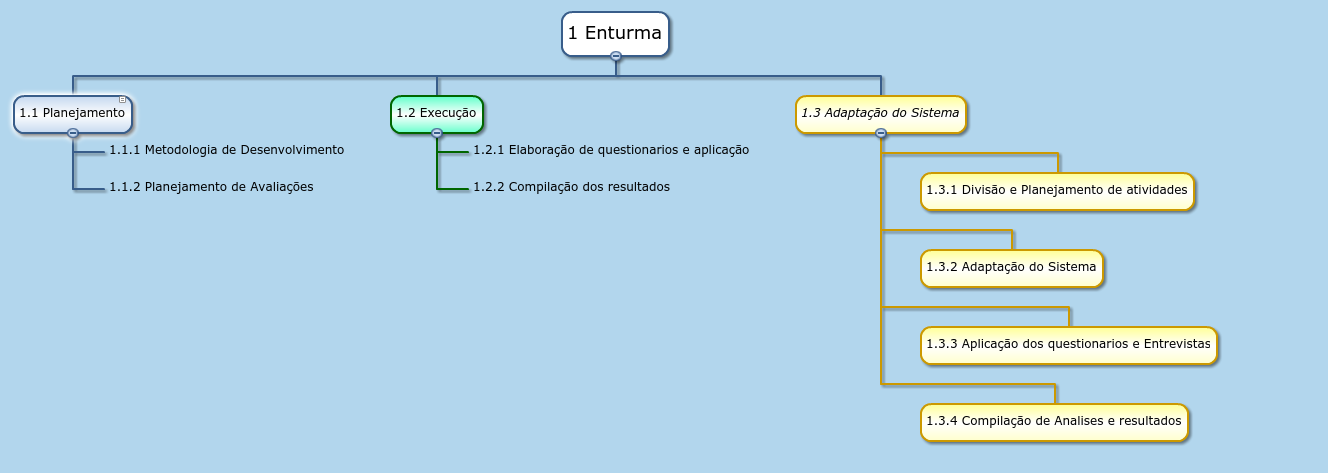
\includegraphics[width=1\textwidth]{imagens/EAP}
		\caption{EAP do Projeto}
		\label{img:EAP}
	\end{figure}
	
	

\subsection{5.3. Lista de software}
	
	Durante o processo de Avaliação do Sistema Enturma, que engloba desde o Planejamento da Avaliação até a Análise dos Resultados obtidos, serão usados diversos \textit{softwares} e tecnologias para apoiar a Equipe, tais como:

	\begin{table}[H]
		\centering
		
		\label{tecnologias}
		\begin{tabular}{|l|l|lll}
			\cline{1-2}
			{\bf Tecnologia} & {\bf Utilidade}                                                                                          & {\bf } &  &  \\ \cline{1-2}
			{\bf GIT}        & O sistema Git será utilizado para Controle de Versões durante o projeto.      &        &  &  \\ \cline{1-2}
			{\bf GitHub}     & Será utilizado como repositório remoto do GIT           &        &  &  \\ \cline{1-2}
			{\bf LaTeX}      & Utilizado para o desenvolvimento de toda a documentação durante a execução do projeto. &        &  &  \\ \cline{1-2}
			{\bf Sublime}    & Será utilizado como IDE para a Documentação e Evolução do sistemaEnturma.   &        &  &  \\ \cline{1-2}
			{\bf GITTER}     & Será utilzado para comunicação, via GitHub, da Equipe.                 &        &  &  \\ \cline{1-2}
			{\bf ASES}       & Será utilizado para Avaliação da Acessibilidade do Sistema Enturma. &        &  &  \\ \cline{1-2}
			{\bf LibreOffice Calc}       & Será utilizado para desenvolvimento do RoadMap e Cronograma &        &  &  \\ \cline{1-2}
		\end{tabular}
		\caption{Tecnologias Utilizadas}
	\end{table}

\subsection{Cronograma de Atividades}

	O Cronograma do Projeto pode ser obtido acessando o < link https://docs.google.com/spreadsheets/d/ \\ 1uaGUFw3tpqgcV94JXcte\_O7jXWjGxHUPm23UfJ4OCh8 >. Como representação, segue a parte inicial do Cronograma de Atividades:

	\begin{figure}[H]
		\centering
		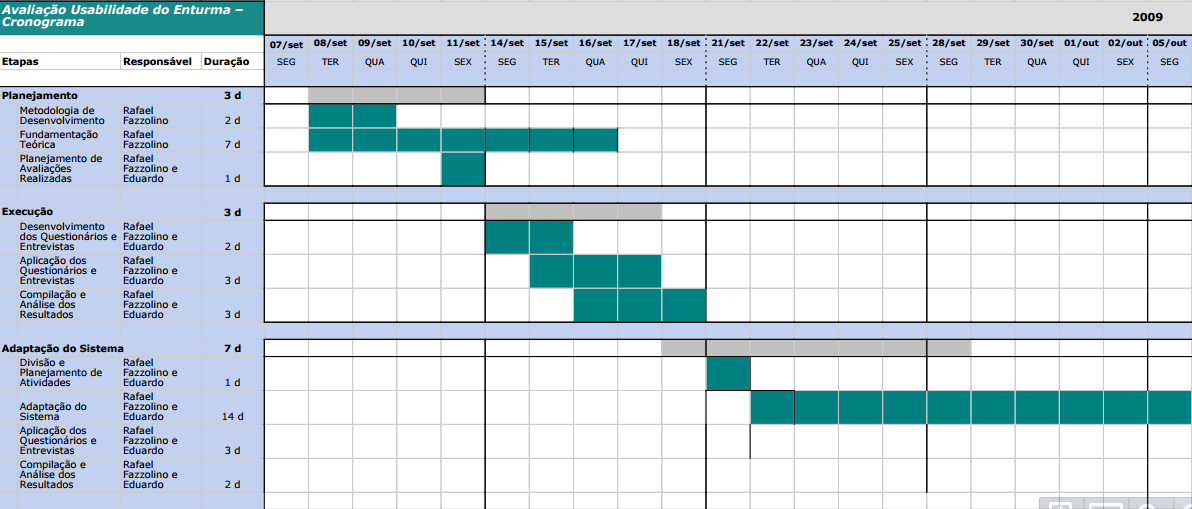
\includegraphics[width=1\textwidth]{imagens/cronograma}
		\caption{Cronograma Inicial do Projeto}
		\label{img:cronograma}
	\end{figure}

